\documentclass{ArticleUSP}

\addbibresource{bibliografia.bib}

%% Dados universidade
\universidade{Universidade de São Paulo}
\faculdade{Escola de Engenharia de São Carlos}
\cidade{São Carlos}

\titulo{Projeto de Aprendizado de Máquina}
\entregaProjeto{Primeira entrega}
\modalidadeProjeto{de relatório científico}
\disciplina{Aprendizado de Máquina}{SCC0276}

\membroA{Calvin Suzuki}{11232420}
\membroB{Guilherme Soares Silvestre}{11299832}
\membroC{Vitor Fernando Rinaldini}{11232305}

\professor{Fernando Pereira dos Santos}{Prof.}

\begin{document}

\pagenumbering{roman}

\geraTitulo

% \begin{resumo}

%   Texto

%   \palavraschaves{\textit{Smart glasses}, Aplicação cirúrgica, Visão computacional, Realidade aumentada}
  
% \end{resumo}

\clearpage

\tableofcontents

\thispagestyle{empty}

\clearpage

\pagenumbering{arabic}

 \chapter{Introdução}\label{chp:intro}

Usinas hidrelétricas respondem pela maior parte da geração energética do Brasil, de modo que a otimização do rendimento dessas plantas é fundamental para manter a estabilidade da rede, preservando os níveis de água dos reservatórios, e diminuindo o custo de operação.
No presente trabalho, busca-se fazer uma análise multidimensional dos parâmetros de projeto de uma turbina Francis, desde a econometria por trás da implementação nessa escala até a modelagem do funcionamento e dimensionamento de parâmetros gerais da turbina, visando otimizar o rendimento energético mecânico.
Serão avaliados também os impactos de parâmetros críticos na eficiência do sistema, direcionando as escolhas do projeto.

\chapter{\textit{Datasets}}\label{chp:datasets}

\section{Obtenção e pré-processamento dos dados}

Os \textit{datasets} presentes na literatura são obtidos a partir da colagem de eletrodos em diversos locais na escalpe do indivíduo para a obtenção dos dados, resultando em um registro de vários sinais de tensão cerebral em um intervalo de tempo. Cada \textit{dataset} possui seus próprios parâmetros como: taxa de amostragem; tamanho do intervalo; quantidade de eletrodos; e etc. Vale salientar que esses valores requerem pré-processamento antes de serem utilizados e validados por um método de aprendizado, por exemplo, para remoção de ruídos oriundos da imprecisão técnica do aparelho ou oscilações na rede elétrica.

No processo de limpeza são utilizados filtros de passa-alta, removendo componentes CC dos sinais e também os desvios, e de passa-baixa, eliminando as peças de alta frequência dos dados. Além dessas, também podem ser aplicadas outras formas, dependendo das imprevisões ocorridas durante a etapa de monitoramento. Um exemplo é a aplicação da técnica de correção de artefatos de Eletrooculograma (EOG), que pode ser necessário se o sujeito sob gravação estiver com os olhos aberto. \cite{EEGMANIQUINS}

\begin{figure}[!h]
    \centering
    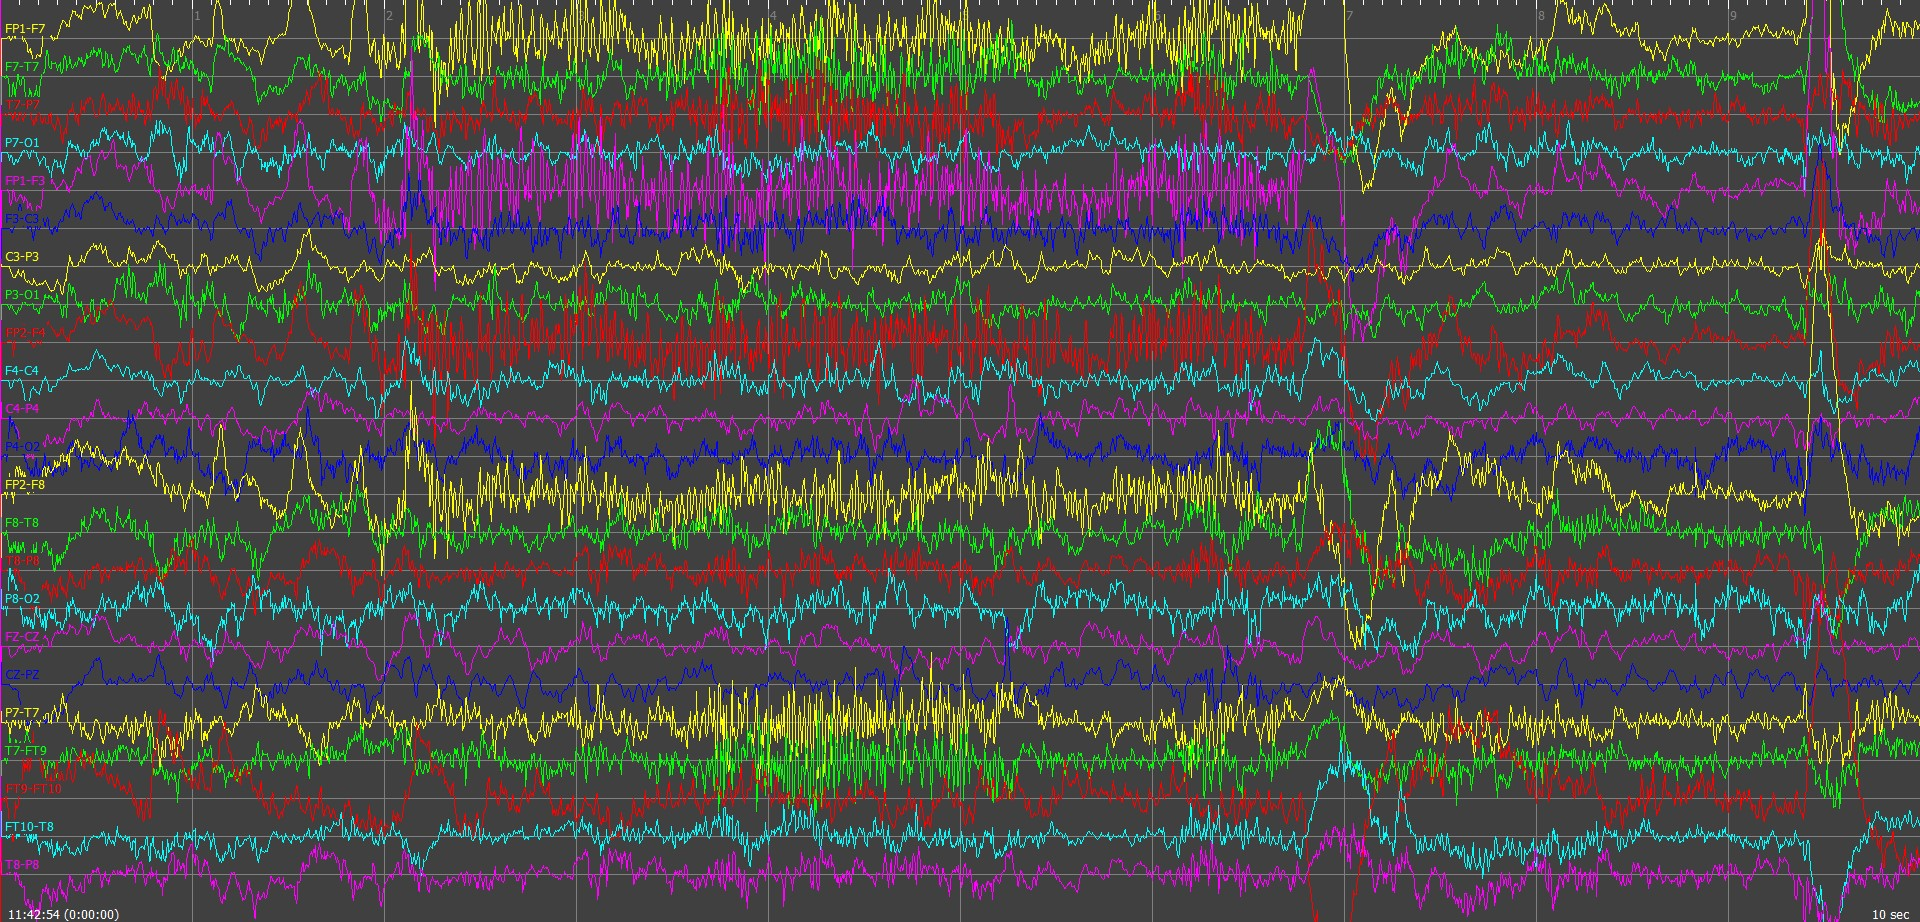
\includegraphics[width=0.7\textwidth]{figuras/exemplo_eeg.jpg}
    \caption{Exemplo de um Eletroencefalograma (EEG).}
    \label{fig:exemplo_eeg}
\end{figure}

O próximo procedimento é a interpretação dos dados e, consequentemente, a extração de recursos. Dado um EEG, essa tarefa é complicada para ser realizada a olho nu (figura \ref{fig:exemplo_eeg}). Exatamente por isto, foram desenvolvidos vários algoritmos complexos de processamento que fazem esse procedimento e separam as características no domínio do tempo e da frequência.

Como resultado da etapa anterior, deve-se obter uma alta gama de propriedades. Devido a isto, se faz necessário um procedimento de seleção de recursos, visando buscar apenas as características necessárias para a modelagem do problema.

Somente após a execução dos roteiros anteriores, os dados estarão prontos para alimentarem nossos modelos de aprendizado de máquina. Vale ressaltar que os processos de obtenção requerem anos ou até mesmo décadas para que acumulem uma quantidade suficiente de valores e, com isso, possibilitar a alimentação dos algorítimos. Entretanto, isso é algo que vem sendo armazenado há muito tempo e a melhor parte é que está disponível ao público. Na próxima seção, falaremos dos \textit{datasets open-sources} existentes na internet.

\section{Datasets existentes}

\subsection{CHB-MIT Scalp EEG \textit{Database}}

Esse banco de dados, consiste em registros de EEG de pacientes pediátricos com convulsões intratáveis. Os indivíduos foram monitorados por vários dias e, após a retirada da medicação anticonvulsivante, caracterizamos suas convulsões e avaliamos sua candidatura à intervenção cirúrgica \cite{CHB-MIT}.

%falar como os dados estão organizados
Todos os sinais foram coletados em 256 amostras por segundo com resolução de 16 bits. A maioria dos arquivos contém 23 sinais de EEG (24 ou 26 em alguns casos). O sistema \textit{International 10-20} de posições e nomenclatura dos eletrodos de EEG foi usado para esses registros.

\subsection{Outros \textit{datasets}}

Existe um repositório no \textit{GitHub} com uma ampla quantidade de \textit{datasets} sobre EEG's \cite{GITREPOSITORIO} que estão separados por categorias como Motor-Imagem; Emoção-Reconhecimento; Potenciais Relacionados a Erros; e entre outros. Destacamos a possibilidade de utilizarmos o \textit{dataset} de convulsões, visto que ela é um dos principais sintomas da crise epiléptica. Obviamente, devemos lembrar que uma pessoa pode não apresentar esse sintoma durante um ataque, portanto esse banco de dados sozinho é ineficiente para o treinamento, contudo, ainda podemos utilizá-lo para testar a acurácia do modelo, após treinado.

\chapter{\textit{Benchmarks}}\label{chp:benchmk}

\subsection{Plataformas}

Infelizmente não se apresentam na comunidade e na literatura grandes quantidades de \textit{benchmarks} contendo os trabalhos que foram desenvolvidos e os resultados alcançados. Entretanto, existem algumas plataformas que estão crescendo e apresentam a tarefa de detecção de crises epilépticas com alguns trabalhos catalogados. Entre elas o \textit{Papers With Code} \cite{paperswithcode}, ou também o \textit{Kaggle} \cite{kaggle}. 

\subsection{Métricas}

Para avaliar os modelos, a literatura utiliza métricas como a taxa de acertos, os falsos positivos e falsos negativos \cite{godoyprediccao}. Já que a tarefa é uma classificação binária, os meios de avaliação da resposta são mais simples em relação a outras tarefas de aprendizado de máquina. Além disso, métodos de avaliação dos modelos como a complexidade, a curva de treinamento e a avaliação de hiper-parâmetros permitem a análise mais aprofundada do modelo e promove consequências diretas nos resultados.

\chapter{\textit{Proposta}}\label{chp:proposta}

Portanto, pretendemos aplicar os diferentes métodos de aprendizado de máquina para detectar momentos de uma crise epilética. Ao final, iremos comparar a acurácia e a complexidade de cada método para esse determinado problema e discutir dos resultados obtidos.

Por fim, Vale salientar que o objetivo é fazer uma classificação binária em positivo ou negativo para um processo epiléptico dado diversos intervalos diferentes de tempo. O resultado esperado está representado na figura \ref{fig:binary_class}.

\begin{figure}[!h]
    \centering
    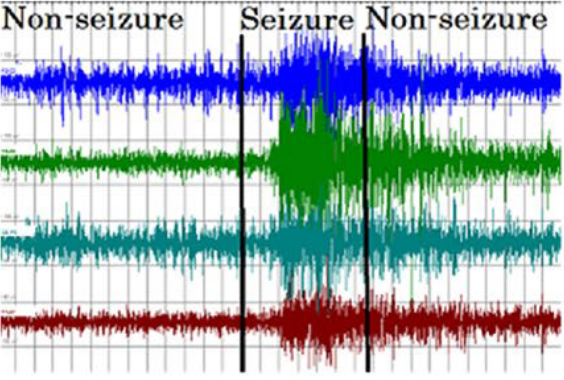
\includegraphics[width=0.4\textwidth]{figuras/binary_class.png}
    \caption{Classificação binária em uma amostra EEG}
    \label{fig:binary_class}
\end{figure}

% Referências bibliográficas
\printbibliography[heading=bibintoc, title={Referências bibliográficas} ]

\end{document}